\subsection{Factor Graphs}
Factor graphs provide a formal framework for representing probabilistic relationships between system variables and sensor measurements. The system is expressed as a collection of local factors, each describing a specific probabilistic constraint such as a motion model, measurement model, or prior. Instead of working with the complete joint probability distribution, which is often high dimensional and computationally expensive, the estimation problem is decomposed into smaller, locally defined probability functions. Each factor depends only on the subset of variables relevant to that constraint, allowing independent evaluation and efficient combination of information from different parts of the system. This structure is conceptually related to the Hidden Markov Model discussed in the following chapter on State Estimation, where states are conditionally dependent over time. However, the factor graph provides a more general formulation that can represent arbitrary dependencies between variables, making it a suitable mathematical framework for expressing probabilistic relationships in problems such as SLAM and other state estimation tasks.
\\ \\
In this work, the factor graph is used to represent the relationships between the microAmpere ASV state variables and their associated sensor data for SLAM problem. The INS motion model defines the motion factors that connect consecutive time steps, while the processed Side Scan Sonar observations provide measurement factors that relate observed features to the estimated trajectory. This formulation gives a clear and consistent way to integrate different sensing modalities within one unified probabilistic system model.  
\\ \\
The factor graph structure also forms the basis for optimization based estimation methods used later in Smoothing and Mapping (SAM), where the sparse connections between variables enable efficient computation of the most probable system trajectory.
\begin{figure}[H]
    \centering
    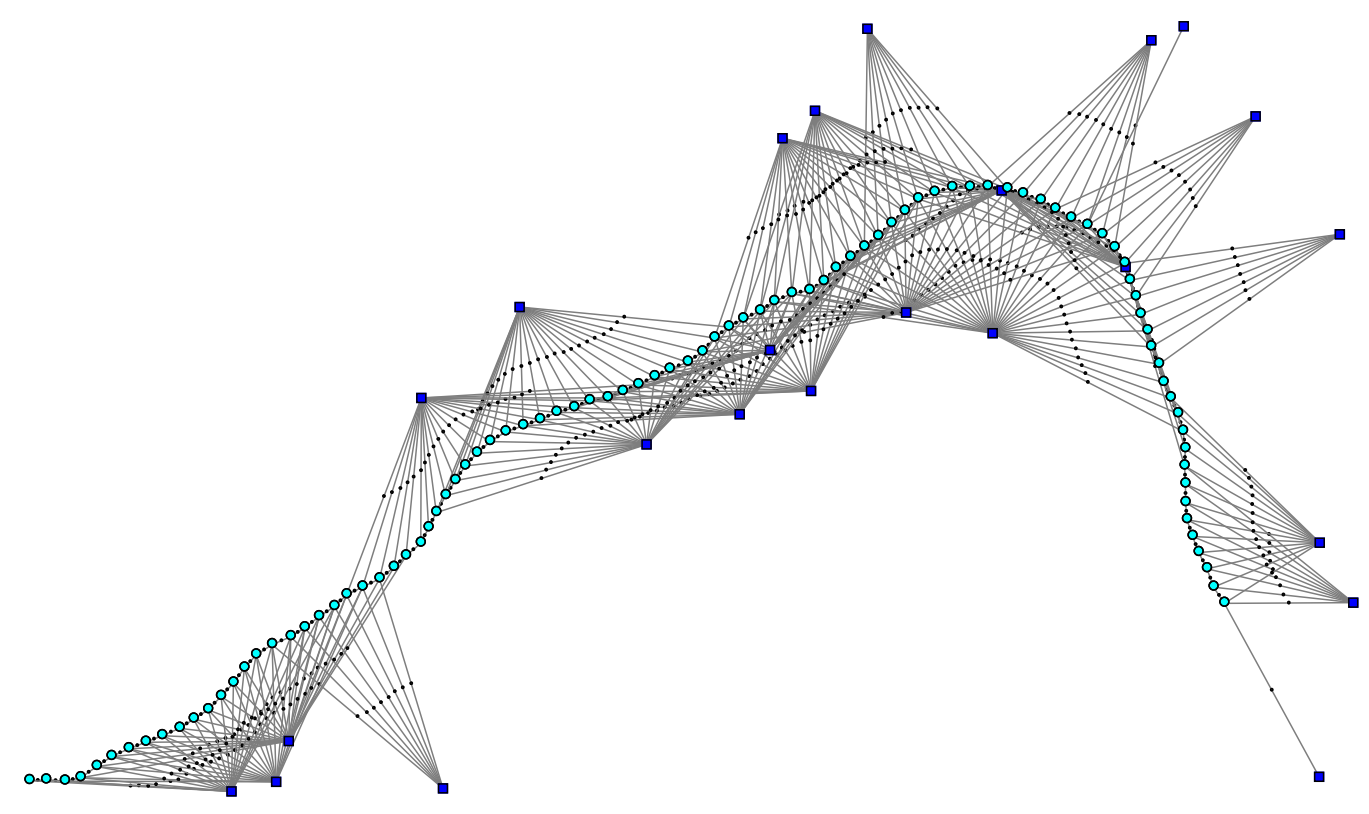
\includegraphics[width=0.9\linewidth]{Pictures/System_Modeling/Factor_Graphs/Example.png}
    \caption{Example of a factor graph in a simulated SLAM problem. Light blue circles represent the estimated robot trajectory, and dark blue squares represent observed landmarks. The connecting black edges/lines are factors, each defining a local probabilistic constraint between variables.\textsuperscript{\cite{factor_graphs}}}
    \label{fig:system-modeling-factor-graph-example}
\end{figure}